\documentclass[11pt,a4paper]{article}

\usepackage[T1]{fontenc}
\usepackage[utf8]{inputenc}
\usepackage{mathpazo}
\usepackage{microtype}
\usepackage[margin=2.4cm]{geometry}
\usepackage{parskip}
\usepackage{amsmath}
\usepackage{xcolor}
\usepackage{colortbl}
\usepackage{booktabs}
\usepackage{multirow}
\usepackage{graphicx}
\usepackage{tikz}
\usetikzlibrary{arrows.meta,positioning}
\usepackage{pgfplots}
\pgfplotsset{compat=1.17}
\usepackage{titlesec}
\usepackage{caption}
\usepackage[colorlinks=true,urlcolor=pkblue,linkcolor=pkblue]{hyperref}

\definecolor{pkred}{RGB}{200,50,60}
\definecolor{pkblue}{RGB}{40,90,160}
\definecolor{pkgrey}{RGB}{90,90,90}

\titleformat{\section}{\large\bfseries\color{pkred}}{}{0pt}{}
\titlespacing*{\section}{0pt}{1.4em}{0.4em}
\captionsetup{font=small,labelfont={bf,color=pkred},justification=raggedright,singlelinecheck=false}
\setlength{\parindent}{0pt}
\renewcommand{\arraystretch}{1.25}

\newcommand{\cell}[2]{\cellcolor{pkblue!#2}#1\%}

\begin{document}
\pagestyle{empty}

{\raggedright
{\Huge\bfseries\color{pkred} Trying to Solve Pok\'emon}\\[0.3em]
{\large\color{pkgrey} How a new hobby turned into a bot-building obsession}\\[0.2em]
{\large\color{pkgrey} (Yes, this is my cover letter. I'm trying to be unique!)}\\[0.2em]
\rule{\linewidth}{0.6pt}
}

\vspace{0.6em}

%% ------------------------------------------------------------------
\section*{How it started}

A new hobby I've picked up in the last month is competitive Pok\'emon, specifically VGC, the official doubles format where you bring four of your six Pok\'emon and fight with two at a time. I guess since there are no more competitive programming contests for me at uni, I've been missing the competitiveness of it all (not the programming??). Turns out I'm pretty good at it, too since I climbed into the top 5,000 players in the world within a month.

Anyway, Pok\'emon is a turn-based PvP game, so on paper it looks a lot like chess. Which got me wondering, how would I solve Pok\'emon with a bot? Ahh, there comes out my programming side.

\IfFileExists{vgc_battle.png}{%
\begin{figure}[h]
\centering
\includegraphics[width=0.8\linewidth]{vgc_battle.png}
\caption{A VGC doubles battle on Pok\'emon Showdown (my own screenshot).}
\end{figure}
}{}

%% ------------------------------------------------------------------
\section*{Attempt \#1: minimax (a.k.a.\ my chess brain)}

So I started building a Pok\'emon bot. I've coded a chess bot before, so I reached for the technique I already knew -  \textbf{minimax with alpha-beta pruning}. Minimax pictures the game as a tree of possible futures. You pick the move that leads to the best outcome \emph{assuming your opponent always replies with the move that's worst for you}, and alpha-beta pruning skips branches that provably can't change the answer, which is what makes it fast enough for chess.

In a format with open team sheets (both players see the opponent's six Pok\'emon, items, abilities, moves and Mega evolutions before the battle) this sounded like a surefire way to find the best move every turn. Turns out it's much harder in practice, for three reasons.

\textbf{1.\ Damage is random.} The damage a move does isn't fixed. In the current games it comes from this formula (with a few rare multipliers left out):
\begin{multline*}
\text{Damage} = \left(\dfrac{\left(\frac{2L}{5}+2\right)\cdot P\cdot \frac{A}{D}}{50}+2\right)\\
\times\, \text{Targets}\times\text{Weather}\times\text{Crit}\times\text{Random}\times\text{STAB}\times\text{Type}\times\text{Burn}\times\text{Other}
\end{multline*}
Here $L$ is the attacker's level (always 50 in VGC), $P$ is the move's base power, and $A/D$ is the attacker's Attack over the target's Defense (or Sp.\ Atk over Sp.\ Def for special moves). Those stats come from yet another formula involving base stats, EVs, IVs and nature: for a non-HP stat, $\lfloor(\lfloor(2B+\text{IV}+\lfloor\text{EV}/4\rfloor)\cdot L/100\rfloor+5)\cdot\text{nature}\rfloor$. The multipliers are:
\begin{itemize}\setlength\itemsep{0pt}
\item \textbf{Targets}: $0.75$ if the move hits more than one target (spread moves in doubles), otherwise $1$.
\item \textbf{Weather}: $1.5$ or $0.5$, e.g.\ Fire moves in sun or Water moves in rain.
\item \textbf{Crit}: $1.5$ on a critical hit (older generations used $2$). The base crit chance is $1/24$.
\item \textbf{Random}: an integer from $85$ to $100$, divided by $100$. There are 16 equally likely rolls, so a move does somewhere between 85\% and 100\% of its maximum damage.
\item \textbf{STAB}: $1.5$ if the move matches one of the attacker's types.
\item \textbf{Type}: $0$, $0.25$, $0.5$, $1$, $2$ or $4$ depending on type matchups.
\item \textbf{Burn}: $0.5$ for physical moves from a burned attacker.
\item \textbf{Other}: items, abilities, screens like Reflect, and so on.
\end{itemize}
Every intermediate step is also rounded down in-game, which is why serious damage calculators exist. The upshot is that you can never be sure exactly how much damage a move will do, and on top of the damage roll there are misses, flinches, and secondary effects. Handling this means adding \emph{chance nodes} to the tree (an extension called expectiminimax), which makes it much bigger.

\begin{figure}[h]
\centering
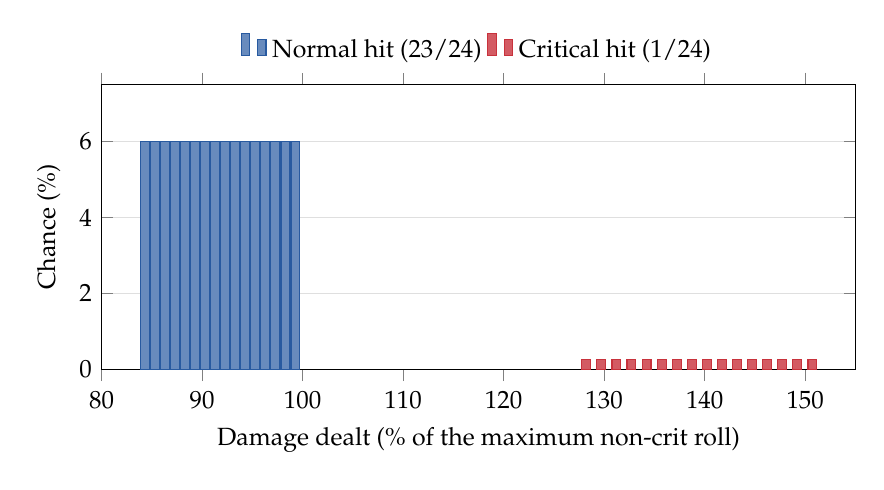
\begin{tikzpicture}
\begin{axis}[
    width=0.92\linewidth, height=5.2cm,
    ybar, bar width=3.2pt,
    xmin=80, xmax=155, ymin=0, ymax=7.5,
    xlabel={Damage dealt (\% of the maximum non-crit roll)},
    ylabel={Chance (\%)},
    legend style={at={(0.5,1.04)},anchor=south,draw=none,legend columns=-1,font=\small},
    tick label style={font=\small}, label style={font=\small},
    ymajorgrids, grid style={gray!25},
]
\addplot+[fill=pkblue!70,draw=pkblue,samples=16,domain=85:100] {5.99};
\addplot+[fill=pkred!80,draw=pkred,samples=16,domain=127.5:150] {0.26};
\legend{Normal hit (23/24),Critical hit (1/24)}
\end{axis}
\end{tikzpicture}
\caption{All 32 possible damage outcomes of a single move: 16 damage rolls, with or without a critical hit. A crit pushes every roll up by 1.5$\times$, but happens rarely, so the bars are tiny.}
\label{fig:dmg}
\end{figure}

\textbf{2.\ ``Open'' isn't fully open.} Even with open team sheets, the sheet doesn't list natures or EV spreads, so I can't calculate my opponent's stats exactly and my damage numbers turn into ranges. I also don't know which four of their six Pok\'emon they'll actually bring. So there's still hidden information.

\textbf{3.\ Both players move at the same time.} This is the big one. Unlike chess, both players lock in their moves simultaneously, so my best move depends on what my opponent picks, and \emph{their} best move depends on mine. It's rock-paper-scissors with health bars. Minimax is built for alternating turns, and alpha-beta pruning doesn't carry over cleanly to simultaneous moves. In doubles it's even worse: you choose an action for each of your two Pok\'emon every turn (moves, targets, switches, mega evolving), which easily gives well over a hundred options per side. Multiply that out with damage rolls and the tree explodes.

\begin{figure}[h]
\centering
\begin{tabular}{@{}ll|ccc@{}}
 & & \multicolumn{3}{c}{\textbf{Opponent plays\ldots}}\\
 & & \textbf{Attack} & \textbf{Protect} & \textbf{Set up}\\ \cmidrule{2-5}
\multirow{3}{*}{\rotatebox{90}{\textbf{I play\ldots}}} &
\textbf{Attack}  & \cell{50}{20} & \cell{30}{5}  & \cell{70}{60}\\
& \textbf{Protect} & \cell{60}{40} & \cell{50}{20} & \cell{30}{5}\\
& \textbf{Set up}  & \cell{35}{10} & \cell{65}{55} & \cell{50}{20}\\
\end{tabular}
\caption{A toy one-on-one turn, with made-up chances that \emph{I} win. Attack gets blanked by Protect, Protect lets a Set-up go through for free, and Set-up gets punished by Attack, so every row has a counter. The best single move only guarantees me 35\%, but randomising about 31/37/33 across the three guarantees 48.8\% against anything.}
\label{fig:matrix}
\end{figure}

That last point is the real kicker. There usually isn't a single ``optimal move'' at all. In a two-player zero-sum game like this, the minimax theorem guarantees an \emph{optimal strategy}, but it's a probability distribution over moves, not one move (Figure~\ref{fig:matrix}). Being unpredictable is literally part of playing optimally. So how do you solve that?

%% ------------------------------------------------------------------
\section*{Enter reinforcement learning}

Enter reinforcement learning (RL), at least that's what I've found out so far. The idea is refreshingly simple: instead of searching through possibilities during the battle, you let a neural network play an enormous number of battles, mostly against copies of itself, and learn from the results.

\begin{figure}[h]
\centering
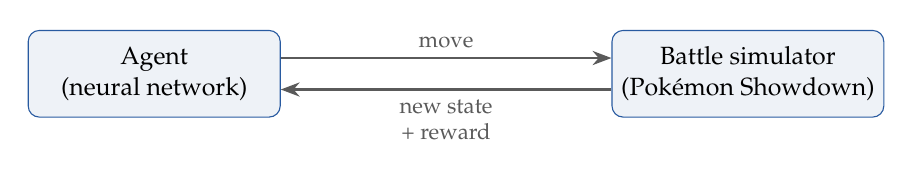
\begin{tikzpicture}[
  node distance=2.6cm,
  box/.style={draw=pkblue,fill=pkblue!8,rounded corners,minimum width=3.2cm,minimum height=1.1cm,align=center,font=\small},
  arr/.style={-{Stealth[length=2.4mm]},thick,pkgrey}]
\node[box] (agent) {Agent\\(neural network)};
\node[box,right=4.2cm of agent] (env) {Battle simulator\\(Pok\'emon Showdown)};
\draw[arr] ([yshift=0.2cm]agent.east) -- node[above,font=\footnotesize]{move} ([yshift=0.2cm]env.west);
\draw[arr] ([yshift=-0.2cm]env.west) -- node[below,font=\footnotesize,align=center]{new state\\+ reward} ([yshift=-0.2cm]agent.east);
\end{tikzpicture}
\caption{The RL loop. The agent plays, sees what happens, and learns from the outcome.}
\end{figure}

After every game the bot gets a reward (say $+1$ for a win and $-1$ for a loss) and tweaks its weights so the choices that led to wins become more likely next time; PPO is a popular algorithm for this. What it ends up learning is a \emph{policy}: a function from ``what I can see right now'' to a probability distribution over moves. That's exactly what a simultaneous-move game needs, since being unpredictable is part of playing well. It also learns a \emph{value estimate}, ``how likely am I to win from here?'', which replaces the evaluation function I'd otherwise have to hand-craft. The catch is that a win only shows up at the end of a game, so the bot has to work out which of the previous 10--15 turns actually mattered (the \emph{credit assignment} problem), and that takes millions of games.

I'm obviously not the first person to have this idea. Open-source bots like Foul Play and Metamon\footnote{Foul Play: \url{https://github.com/pmariglia/foul-play}. Metamon: \url{https://metamon.tech}.} have climbed high up the Pok\'emon Showdown ladders in singles formats, good enough to beat most human players. But they're far from the final word, and most of the open-source work I've found is for singles, so there's a lot left to improve, especially for doubles. Right now I'm teaching myself RL so I can build something like that myself.

%% ------------------------------------------------------------------
\section*{Search isn't dead yet}

None of this means minimax-style search is obsolete. Funny enough, Foul Play isn't an RL bot at all, it's apparantly search-based, and it started out using minimax. Its author swapped minimax for Monte Carlo tree search specifically because it copes better with simultaneous moves, which is the exact problem I just spent half this essay complaining about. So my chess brain wasn't entirely wrong, just a few upgrades short.

It also shows up at the very top of the human game. Wolfe Glick (WolfeyVGC), the 2016 World Champion and often called one of the best VGC players ever, apparently has a ``special technique'' he saves for tournament finals: the night before, he maps out all the possible lines of play by hand and picks the road to victory that holds up best. That is literally a game-tree search done on paper. According to him it's extremely time-consuming, so he can only do it for finals, where he knows his opponent's team a whole day in advance. With a minimax-style algorithm, that same exercise takes a lot less time, and it could be done for any match.

So that's where I'm at on my competitive pokemon journey - a month into competitive Pok\'emon, a pile of half-working code, and a reading list that keeps growing. Worst case, I learn a lot about reinforcement learning. Best case, I build a bot that out-predicts me. Oh my, did I forget to actually play the game?

\end{document}